\documentclass{minimal}
\usepackage{graphicx,color}
\usepackage[papersize={576.00bp,432.00bp},text={576.00bp,432.00bp}]{geometry}
\begin{document}
\centering
% Title: gl2ps_renderer figure
% Creator: GL2PS 1.4.0, (C) 1999-2017 C. Geuzaine
% For: Octave
% CreationDate: Tue Sep 25 18:21:35 2018
\setlength{\unitlength}{1pt}
\begin{picture}(0,0)
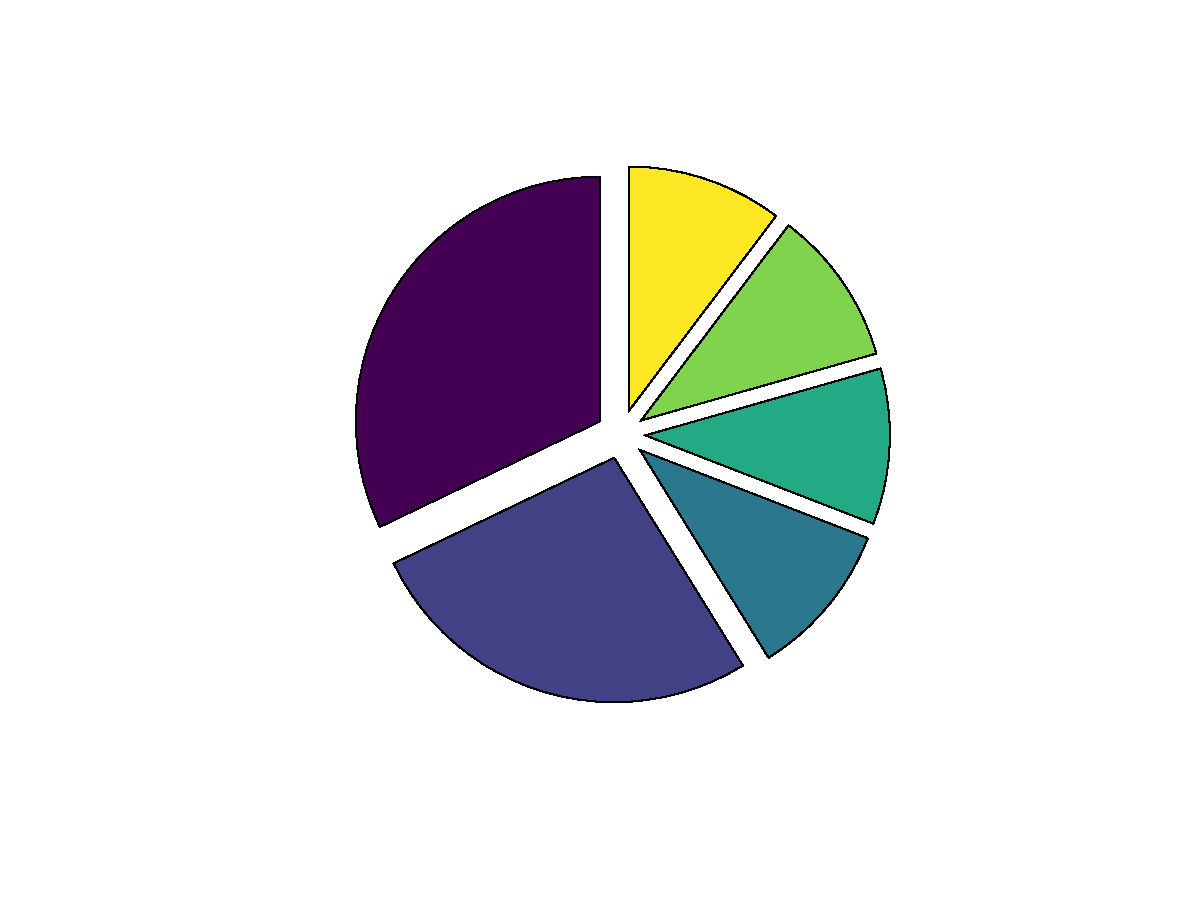
\includegraphics{roba_exito_rank-inc}
\end{picture}%
\begin{picture}(576,432)(0,0)
\fontsize{11}{0}
\selectfont\put(298.08,409.6){\makebox(0,0)[b]{\textcolor[rgb]{0,0,0}{{Ranking de Roba Éxito con p = 0.65}}}}
\fontsize{10}{0}
\selectfont\put(178.899,298.59){\makebox(0,0)[r]{\textcolor[rgb]{0,0,0}{{Nodo 1 - 0.32115}}}}
\fontsize{10}{0}
\selectfont\put(258.53,88.3956){\makebox(0,0)[r]{\textcolor[rgb]{0,0,0}{{Nodo 2 - 0.26708}}}}
\fontsize{10}{0}
\selectfont\put(406.427,133.59){\makebox(0,0)[l]{\textcolor[rgb]{0,0,0}{{Nodo 3 - 0.10294}}}}
\fontsize{10}{0}
\selectfont\put(438.762,217.056){\makebox(0,0)[l]{\textcolor[rgb]{0,0,0}{{Nodo 4 - 0.10294}}}}
\fontsize{10}{0}
\selectfont\put(414.266,303.149){\makebox(0,0)[l]{\textcolor[rgb]{0,0,0}{{Nodo 5 - 0.10294}}}}
\fontsize{10}{0}
\selectfont\put(342.835,357.091){\makebox(0,0)[l]{\textcolor[rgb]{0,0,0}{{Nodo 6 - 0.10294}}}}
\end{picture}
\end{document}
